\documentclass{acm_proc_article-sp}
\usepackage{times}
\usepackage{url}
\usepackage{graphics}
\usepackage{color}
\newcommand{\want}[1]{}
\newcommand{\idea}[1]{}
\newcommand{\note}[1]{}
%\newcommand{\x}[1]{}
\newcommand{\todo}[1]{}
\newcommand{\maybe}[1]{}
\newcommand{\resolved}[1]{}

% Mark up a point that we want to flesh out into more text
\newcommand{\x}[1]{{\color{blue} #1}\\}

% Mark up some work that we need to do in order for this paper to be telling the truth
%\newcommand{\todo}[1]{{\color{red} #1}\\}

%\newcommand{\maybe}[1]{}

\begin{document}

\toappear

\bibliographystyle{plain}

\title{What is disputed on the web?}

%%
%% Note on formatting authors at different institutions, as shown below:
%% Change width arg (currently 7cm) to parbox commands as needed to
%% accommodate widest lines, taking care not to overflow the 17.8cm line width.
%% Add or delete parboxes for additional authors at different institutions. 
%% If additional authors won't fit in one row, you can add a "\\"  at the
%% end of a parbox's closing "}" to have the next parbox start a new row.
%% Be sure NOT to put any blank lines between parbox commands!
%%

\numberofauthors{5}

\author{
\alignauthor Rob Ennals\\
       \affaddr{Intel Labs Berkeley}\\
       \affaddr{2150 Shattuck Ave}\\
       \affaddr{Berkeley, CA, USA}\\
       \email{robert.ennals@intel.com}
\alignauthor Dan Byler\\
       \affaddr{School of Information}\\
       \affaddr{University of California at Berkeley}\\
       \affaddr{Berkeley, CA, USA}\\
       \email{daniel.byler@berkeley.edu}
\and
\alignauthor John Mark Agosta\\
       \affaddr{Intel Labs Santa Clara}\\
       \affaddr{2200 Mission College Blvd}\\
       \affaddr{Santa Clara, CA, USA}\\
       \email{john.m.agosta@intel.com}
\alignauthor Barbara Rosario\\
       \affaddr{Intel Labs Santa Clara}\\
       \affaddr{2200 Mission College Blvd}\\
       \affaddr{Santa Clara, CA, USA}\\
       \email{john.m.agosta@intel.com}
}

%\sloppy


\maketitle

%RULE: Don't cite media reports unless I have to - some reviewers don't like it


\abstract

We present a method for the automatic acquisition of a corpus of disputed claims from the web. We consider a claim to be disputed if a page on the web suggests that this claim is wrong and that other people on the web are suggesting that it is true.

Our tool extracts disputed claims by searching the web for patterns such as ``falsely claimed that $X$'' and then using a statistical classifier to select text that appears to be making a disputed claim. 

We argue why such a corpus of dispupted claims is useful for a wide range of applications related to information credibility on the web, and we look at what our current corpus reveals about what is being disputed on the web.

\resolved{too much emphasis on {\em how}... rewrite following paragrapgh}

%\subsection{Categories and Subject Descriptors}
%\todo{Categories, terms, and keywords need updating}
\category{H.3.1}{INFORMATION STORAGE AND RETRIEVAL}{Content Analysis and Indexing}
\category{I.2.7}{ARTIFICIAL INTELLIGENCE}{Natural Language Processing}

\terms{Design, Human Factors}

\keywords{Sensemaking, Annotation, Argumentation, Web, CSCW}

\tolerance=400 
  % makes some lines with lots of white space, but  
  % tends to prevent words from sticking out in the margin

\section{Introduction}

The web contains a vast number of pages written by a vast number of people. In many cases, these people disagree with each other, and the pages they write contain conflicting information. For users to extract reliable information from the web, it is useful for them to be able to determine when different sources disagree about a topic.

In this paper we describe a method for automatically acquiring a corpus of disputed claims from the web. We consider a claim to be {\it disputed} if a page exists on the web that suggests both that the claim is false, and that there are others that are making the claim. We are also interested in {\it who} disputes a particular claim, since a user is likely to be more interested in being told that a claim is disputed by a large number of sources that they believe are credible, rather than a small number of sources that they do not trust.

We identify disputed claims by searching for lexical patterns such as ``the misconception that $S$'' (Section~\ref{findingclaims}). For example, if a page contains the text ``the minconception that {\it the moon is made of cheese}'', this suggests that the author believes that others are saying that the moon is made of cheese, and that the author themselves disputes this claim. In Figure~\ref{templates} we list some of the patterns we used. In practice, many of the strings that match such a pattern are not well-formed disputed claims. We use a statistical classifier to filter out those strings that appear to make a well-formed claim.

We believe that this corpus will be useful for many purposes. We are currently using it as part of our Dispute Finder~\cite{Ennals2010} project to automatically highlight phrases on web pages that are disputed by other sources. We are also exploring other applications of this corpus, including automatically detecting disputed claims in human speech, and visualization tools that let users know what is disputed about a topic that interests them, and statistical tools that allow people to look for patterns in internet debate  (Section~\ref{using}).

We have made our corpus publicly available for other researchers to download at \url{http://confront.intel-research.net/}. In currently contains claims extracted from pages written on the days between October 1st 2009 and January 19th 2010, and pages written on January 10th of every year from 2000 to 2010. This amounts to approxmately 1.1 million strings that we believe are making disputed claims. We plan to expand our corpus as we crawl more of the web and improve our algorithms.

By looking at the claims in this corpus, we see trends in dispute on the web that correspond to the debates that were particulary topical at particular times (Section~\ref{analysis}).

We believe that ours is the first attempt to automatically acquire a corpus of disputed claims from the Web.


\section{Background and Related Work}

The problem of determining information credibility on the web is becoming increasingly important. In the past a user would typically obtain information from a relatively small set of sources such as books, TV channels, and radio stations. The user would have some idea of the reputation and biases of each of these sources, and publishing barriers and quality control would ensure that these sources only published information that met their standards. 
The web is very different. A user has access to a vast number of different sources, but knows little about the biases or reputation of most of them. Moreover, the internet has little in the way of publishing barriers or quality control. If a user is to extract reliable information from the web, they need to either restrict themselves to a small set of trusted sources, or use some kind of mechanism to determine the credibility of the information that they access.

There are several ways that a user can determine whether to trust information that they find on a web page. The user can check the reputation of the person or organization that wrote the web page; they can check whether the web page looks like a they think a reliable web page should look; or they can check whether the information is consistent with information available from other sources.

A user can check the reputation of a source using a service such as SourceWatch.org, which publishes manually curated information about the reputation and known biases of various sources. Trustpilot.com produce a Firefox extension that warns a user when they are looking at a web page hosted by a company that they believe is not trustworthy. Alternatively, a user can simply use a search engine such as Google to look for information about the source. While these tools can be very useful, trustworthy sources sometimes publish unreliable information, and untrusted sources sometimes contain useful information. For example, a reliable source may have been misled by an unreliable source they were using themselves; or a small unrated blog may publish information that useful, insightful, and accurate. 

Researchers have identified a variety of metrics that can be used to automatically estimate the quality of a document based on looking at its content. For Wikipedia, Blumenstock~\cite{Blumenstock2008} estimates the quality of an article by the word count and WikiTrust~\cite{Adler2008b} identifies potentially unreliable sections of an article by analyzing its edit history. Custard and Sumner~\cite{Custard2005} use a combination of metrics to measure web site quality, including number of links and whether it contains videos. Fogg et al~\cite{Fogg2003} have shown that users commonly evaluate the credibility of a web site based on factors such as the design look, the information structure of the site, and the tone of the writing. Some of the factors identified by Fogg et al could potentially be measured automatically and used to guide a user. These metrics do a good job at detecting pages that resemble pages that contain unreliable information, but they do not protect against authors who write untrustworthy information in the style of a trustworthy document.

In our research, we are following the third approach. We aim to inform users when information that they encounter is disputed by another source. We have built an extension to the Firefox web browser called Dispute Finder~\cite{Ennals2010} that informs users when a web page that they are reading makes a claim that it knows to be disputed. For example, if a user is reading a page that says ``Elvis is Alive'' then Dispute Finder will highlight that statement as being disputed and direct the user to other sources that put forward alternative points of view. In its currently released version, Dispute Finder builds a corpus of disputed claims by allowing users to enter disputed claims manually, and scraping a small set of web sites that manually curate such claims (currently Politifact.org and Snopes.com); however it is difficult to make this approach scale to the huge number of claims on the web that are disputed.

Our primary motivation for automatically acquiring a large corpus of disputed claims is to use this corpus to enable tools like Dispute Finder to automatically inform users when they encounter information that this corpus says is disputed. However, as we discuss in Section~\ref{using}, we believe such a corpus could be useful for many other purposes too.

The problem of detecting disputed claims is closely related to the well-studied problem of detecting contradictions. A claim $H$ is {\it contradicted} if a document somewhere on the web makes a claim that implies that $H$ cannot be true. For example, the claim ``The moon is made of rock'' {\it contradicts} the claim ``The moon is made of cheese''. A contradicted claim is not necessarily a disputed claim. In this example the person who said that the moon was made of rock might not be aware that others think it is made of cheese. A {\it contradiction} is logical, while a {\it dispute} is social. In order for a claim to be disputed, the authors of the documents must be aware that there is a contradiction between their beliefs.

There has been significant work on detecting contradictions. Condoravdi et al~\cite{Condoravdi2003} argue that contradiction detection is one of the key tasks in language understanding. de Marneffe et al~\cite{deMarneffe2008} present a taxonomy of the different ways that claims can contradict each other and describe a system that combines many techniques to detect different kinds of contradictions. AuContraire~\cite{Ritter} uses TextRunner~\cite{Etzioni2008,Banko2008} to infer subject-verb-object relationships, looks for cases where a verb maps the same subject to multiple objects, and uses semantic knowledge to determine when this implies that there is a contradiction. Harabagiu et al~\cite{Harabagiu2006} look for contradictions where one claim is a negated paraphrase of another. The RTE-3 Recognizing Textual Entailment challenge~\cite{Giampiccolo2007} included an optional contradiction detection task, allowing different groups building contradiction detection algorithms to compare their results. 

Detecting contradictions has proven to be a hard problem~\cite{Giampiccolo2007}. Much of the difficulty comes from the fact that one typically needs deep semantic knowledge to determine whether two statements that look like they might contradict each other actually do. For example ``George Bush is married to Barbara Bush'' does not contradict ``George Bush is married to Laura Bush'' because there is more than one George Bush. ``Alan Turing was born in England'' does not contradict ``Alan Turing was born in London'' because London is in England. ``It is raining is San Francisco'' does not contradict ``It is not raining in San Francisco'' if the statements were made at different times. 

We detect disputes rather than contradictions. Rather than looking for claims that contradict each other, we look for evidence that people believe that there is a contradiction and that this contradiction is important. One advantage of looking for disputes rather than contradictions is that this allows humans to do the hard work of identifying contradictions and deciding whether they are important. If a page says ``Falsely claimed that George Bush is married to Barbara Bush'' then that suggests that the contradiction with ``George Bush is married to Laura Bush'' is likely to be genuine. The corresponding disadvantage is that if one looks for disputes, one will only detect contradictions that humans have found and believe are important.

Perhaps more importantly, for our purposes disputes are more interesting than contradictions. We are interested in the social side of dispute. We want to know who disagrees with who, why they disagree, and what they think is important. 

Another closely related area is sentiment analysis/opinion mining~\cite{Hu2004,Pang2004}. Opinion mining tries to determine what an author's opinion is about certain objects or certain features of certain objects. A focal application has been the automatic summarisation of product reviews, to produce an overview of the product features that are viewed favorably or negatively. Dispute mining could be thought of as opinion mining applied to beliefs and ideas, rather than features of objects.

\resolved{All merged? : The methods we use are closely related to related work on information extraction which is the task of identifing and classifing specific semantic entities within documents (i.e. names of locations, people, organizations, temporal expressions etc.) We described such related work in the next Section.}


\section{Finding Disputed Claims}
\label{findingclaims}

\begin{figure}[tb]
\begin{center}
  \begin{tabular}{|lll|}
    \hline
    {\bf Frequency$^*$} & {\bf Template} & {\bf Precision$^\dag$}\\ 
    \hline
        \multicolumn{3}{|c|}{\it Something that could be challenged}\\
        570,000,000 & think that & 28\%\\
        495,000,000 & believe that & 48\%\\
        145,000,000 & idea that & 42\% \\
        101,000,000 & claim that & 46\%\\
       \hline
       \multicolumn{3}{|c|}{\it Something others believe}\\
        40,100,000 & claiming that & 39\% \\
        30,600,000 & the belief that & \\
        28,600,000 & believing that & \\
        11,700,000 & who believe that &\\
        8,400,000 & who think that &\\
        \hline
        \multicolumn{3}{|c|}{\it Something false}\\
        5,790,000 & the myth that & 62\% \\
        3,260,000 & into believing that & 52\% \\
        1,690,000 & the lie that & 52\% \\
        1,410,000 & it is not true that & 64\% \\
        1,220,000 & the delusion that  & 54\%\\
        1,140,000 & the misconception that & 67\%\\
        995,000 & mistaken belief that &\\
        676,000 & the mistaken belief that &\\
        593,000 & mistakenly believe that &\\
        583,000 & the fantasy that &\\
        501,000 & it is not the case that &\\
        459,000 & false claim that &\\
        405,000 & the fallacy that &\\
        351,000 & falsely claimed that &\\
        264,000 & urban legend that &\\
        250,000 & no longer believe that &\\
        216,000 & the false belief that &\\
        215,000 & falsely claiming that &\\ 
        178,000 & falsely believe that &\\
        171,000 & bogus claim that &\\
        163,000 & erroneous belief that &\\
        154,000 & the deception that &\\
        147,000 & the misunderstanding that &\\
        135,000 & urban myth that &\\
    & & \\
    \multicolumn{3}{|l|}{$^*$Yahoo's approximate estimate}\\
    \multicolumn{3}{|l|}{$^\dag$Based on manual inspection of 100 text segments}\\
    \multicolumn{3}{|l|}{\quad matched by each pattern}\\
    \hline
  \end{tabular}
\end{center}

  \label{templates}
  \caption{Patterns we use to find disputed claims}
\end{figure}

We implemented a three stage process to build our corpus of disputed claims, each described in the following Sections. We first create a set of lexical patterns such as ``the misconception that'' and ``it is not the case that'' (Section~\ref{patterns}). We then search the Web for these patterns (Section~\ref{searchpattern}). Finally, we filter the resulting strings to give only those that resemble unambiguous disputed claims (Section~\ref{filterclaim}).

\begin{figure*}[tb]
\begin{center}
\begin{tabular}{|l|l|l|l|}
  \hline
  & {\bf extracted text} & {\bf valid} & {\bf details} \\
  \hline
  1. & the false claim that {\it won't go away} & no & ``wont go away'' is not a statement \\
  2. & falsely claimed that {\it he didn't do it} & no & ``he'' and ``it'' are unbound referents \\
  3. & falsely claimed that {\it federal labor laws do not apply} & no & object of the verb is not present\\
  4. & false claim that {\it Elvis is alive} despite all evidence & yes & but drop everything after ``despite''\\
  5. & wrongly believe that {\it the moon is made of cheese} & yes & it is a statement about the world \\
\hline
\end{tabular}
\end{center}
\label{filtered}
\caption{We filter out text that does not look like a statement}

\end{figure*}

\subsection{Patterns for Finding Claims}
\label{patterns}

\x{Cite Snow on auto-finding new patterns. \cite{Snow2005}}
\x{Cite Ritter on using stats to clean up results. ~\cite{Ritter2009}}
\x{Cite MemeTracker~\cite{Backstrom2009}}

We hand crafted a set of {\bf XX} patterns that we hypothesize may  indicate that a claim is disputed, such as ``false claim that'' or or ``it is not true that.'' 

This is an instance of template inference (aka pattern matching), a method that has been used extensively for many NLP tasks. Hearst~\cite{Hearst1992} searched for templates such as ``$X$ such as $Y$'' to infer hyponyms, Riloff~\cite{Riloff1993} searched for words such as ``kidnapped'' to find information about terrorist events. TextRunner~\cite{Etzioni2008} searches for more general patterns to extract logical relationships from the web.
These methods differ on how {\bf finish here}
\x{add more related work here}
\todo{add more related work here}

In this work we simply start with an initial set of patterns that we wrote by hand. We then found additional templates by searching for the text of known disputed claims, and observing what text commonly occurred as a prefix of a known disputed claim. From this set of candidate prefix patterns, we manually selected additional patterns. 

\x{add more related work on boostraping here, adding differences}
\todo{add more related work here}

We plan to work on more sophisticated algorithms for finding new patterns automatically in future work.

Rather that searching for an arbitrary collection of known disputed claims, we found that we generated better templates by searching for claims that most documents disagee with (e.g. ``eskimos have many words for snow'') rather than claims that many people agree with (e.g. ``there is a God''). If many people agree with a claim is true then many of the patterns that we find will not be patterns that indicate that the claim is disputed. 

We also find that we get higher quality results if we limit ourselves to prefixes that begin with ``that''. For example, if we search for ``that eskimos have many words for snow'' then most prefixes we find do indeed indicate dispute, however if we just search for ``eskimos have many words for snow'' then we get a much lower hit rate. 

\x{not sure if to add what follow, posponing the decision for now}
This approach is an example of the Distributional Hypothesis. The distributional hypothesis, as originally framed~\cite{Harris1954,Systems2000}, theorised that words that appear in similar contexts have similar meanings. This has more recently been extended to patterns. If two patterns appear in a corpus with similar text filling their slots, then it is likely that the patterns have similar meanings. DIRT~\cite{Lin2001} discovers inference rules such as (``$X$ is author of $Y$'' $\equiv$ ``$X$ wrote $Y$'') by looking for patterns that have a similar distribution of text filling their slots. Pasca and Dienes~\cite{Pasca2005} detect paraphrases on the web by searching for text fragments that appear in similar contexts on web pages. 

Figure~\ref{templates} shows a subset of the {\bf xx} patterns  that we used. For each pattern, we show the number of times that Yahoo estimates that the pattern appears on the web. 
\todo{add statistic of patterns and patterna accuracy here}
\x{add statistic of patterns and patterna accuracy here}

Not all patterns have exactly the same meaning. We divide patterns into three fuzzily-grouped categories:

\begin{itemize}
 \item {\bf False:} The author believes the claim is wrong
 \item {\bf Believed by others:} The author believes others think this, and it is likely that the author disagrees. Further inspection is required to determine whether the author disagrees with the claim. 
 \item {\bf Could be challenged:} The author feels the need to state that someone believes something, which suggests that this is something that one might not believe. For example, if an author says ``I think America is a great place'' this doesn't suggest that the claim is false, but the mere fact that they declared that they thought that suggests that they are aware that the claim could be challenged.
\end{itemize}

We grouped patterns into categories by hand, based on a brief inspection of pages that were using each of the patterns. 

Which patterns one should use depends on what one wishes to use the resulting corpus of disputed claims for. If one wants to only have claims for which we can present web pages that argue that the claim is false, then only the first set of patterns should be used. If however one just wishes to see what things people think are worthy of having opinions expressed about, then the full set is useful.
\todo{Give some stats about our patterns}

\subsection{Searching the Web for Claims}
\label{searchpattern}

We then search the web for the set of patterns described in the previous session. Rather than building our own search engine, we use the Yahoo BOSS search API~\cite{yahoo-boss}. We search Yahoo BOSS for a raw string such as ``the misconception that'' and then download every web page that Yahoo lists in its search results.
Since we are using an existing search engine, we are limited to searching for simple text strings. This leads us to generate multiple patterns that are almost the same, other than for synonyms. E.g. ``the lie that'' vs ``the deceit that''. We are also restricted to searching for patterns that consist entirely of either a prefix or a suffix. For example we could not search for ``say that $S$ despite'', because there is no way to require that ``despite'' and ``say that'' be in the same sentence. While we could do the search anyway, and then filter out all pages in which the parts were not in the same sentence, this would be inefficient, since many pages would not contain the pattern.

In the longer term we would like to have a more elegant search infrastructure, but for the time being this approach seems to work reasonably well.

Since we are interested in the time information of the claims and we want to be able to incrementally update our corpus as new pages appear on the web, without repeatedly downloading the same pages, we need to be able to request only pages updated in a given date range. The Yahoo BOSS API does not offer the ability to do so; we thus simulate this behaviour by instead including a literal date string in our queries. For example, if we want to find claims that were disputed on January 4th 2010 then rather than searching for \texttt{``it is not true that''}, we instead search for \texttt{``it is not true that'' ``January 4 2010''}.

The reasoning behind this technique is that many articles on the web include the date the article was posted in the text of the web page, particularly news articles and blog posts. This approach has false positives and false negatives. Some web pages include dates that are not the date the article was posted, and some web pages either don't include the date the article was posted, or write their date in a different format. Indeed our current implementation suffers from a systematic bias towards sites that write their dates in US format (month first) rather than UK format (day first).

\todo{Produce some kind of measure of how well date searching actually works}
\todo{Give some stats about search results}

\subsection{Filtering Statements}
\label{filterclaim}

From the web pages returned from the search, we form a {\it candidate claim} by taking all text from the end of the prefix we searched for, up to the nearest sentence-ending punctuation character or HTML tag (e.g. '.','?','!',\texttt{</p>},\texttt{</h1>}, etc). 

\x{it would be quite important to give a sense on the accuracy --precision - of the claims extracted. you can calculated this from a subset of returned candidate claims: out of, say, 100, how many were actually claims?}

Not every chunk of text identified by one of our patterns is a well-formed disputed claim. Consider for example the text chunks in Figure~\ref{filtered}. A chunk of text might not be a statement (case 1), it might include unbound referents such is ``it'', or ``they'' (case 2), or it might only make sense within the context of a particular document (case 3).

We use a simple filter that looks for cases 1 and 2, but does not yet deal with case 3. We use the part-of-speech tagger from NLTK~\cite{nltk}, and then use a simple regexp parser to apply a series of simple rules.

\begin{enumerate}
\item To ensure that the text represent a real statement (case 1) we accept only text that contains either two noun phrases (e.g. ``{\it George Bush} is from {\it Texas}''), or a noun phrase and an adjective (e.g. ``{\it Cocaine} is {\it addictive}''). We do not accept text that contains merely a noun and a verb (e.g. ``{\it Federal laws} do not {\it apply}'') since manual inspection of our data set suggests that in such phrases the verb typically refers to a noun that is defined outside the statement itself.

\item We also discard any statement that contains a personal pronoun such as ``he'', ``she'', ``it'', or ``they'' unless it is proceeded by a noun (addressing case 2). We allow a personal pronoun after a noun, since manual inspection suggests that in most cases the personal pronoun refers to the noun, for example ``Bill Clinton said he wants to slow down the economy''. While we could in theory resolve other references, this is known to be a hard problem, and we have access to a large enough set of candidate claims that we can afford to throw away claims that are not easy for us to process.

\item In some cases a disputed claim will be followed by information about where the claim was made, or why the claim is wrong. For example ``he claimed that the moon was made of cheese {\it on his show}'' or ``he claimed that the moon is made of cheese {\it despite contrary evidence}''. We chop off such suffixes by discarding any text that follows a word such as ``despite'', ``however'', ``but'', or ``was''.
\end{enumerate}

These rules were crafted by hand, based on trial and error and manual inspection of a relatively small number of claims. In the future we would like to use a more rigorous statistical method to produce more sophisticated rules for selecting high quality disputed claims, guided by a larger hand-annotated data set. We are also considering adopting an external framework such as TextRunner~\cite{Etzioni2008,Banko2008}.
\todo{add related work here}

\todo{Need a rough evaluation of what proportion of claims get thrown away by each rule, and how accurate these rules are.}


\subsection{Context}

\x{Importance of dates}
\x{Work meaning depending on surrounding text}
\x{We do not yet do anything useful with context, but we believe it is important and intend to use it}
\x{context can be surrounding text but also features of the web pages -- domain,  "authority," in-links, format; context is also the author: expert? social info on author...}

\section{Using Disputed Claims}
\label{using}

A corpus of disputed claims could be useful for a variety of applications, including real-time dispute recognition, background dispute analysis agents, and other research tools. Real-time dispute recognition agents could be used, for instance, to alert users when a trusted source disagrees with others, or to provide the user with feedback on how contentious a topic is.

Dispute Finder is one such agent that we are developing to provide real-time dispute recognition to users by identifying disputed claims that appear in web pages. Future iterations of Dispute Finder and other such agents will be designed to work with other media such as television or radio, as well as augmented reality applications. We envision a device that provides real-time feedback to users regarding claims made in a conversation or presentation. Such a device would augment individuals' intuitive recognition of that a disputed claim is being made.

Dispute analysis agents that run in the background represent another application we see for a corpus of disputed claims. Such agents could be trained with information regarding the books, journals, and news articles a user reads. It would then be able to alert the user when a previously-read source is now disputed. It could also track a set of topics and tell the user when something new is disputed about a topic. A background dispute analysis agent would serve as an automated research assistant, alerting me when 

A third category of applications could be broadly classified as research tools: agents which allow users to explore what is disputed about a particular topic, or to more broadly examine the zeitgeist of disputes. In this way the cultural 

Recognizing that these are but a few of the ways in which a disputed claim corpus could be used, we will release this data set to the research community as a whole.

\x{"It will be available for unrestricted use under the XXX license. The dataset can be accessed at http://xxx.intel.com/xxx"}


\section{Analysing the Data}
\label{analysis}

\begin{figure}[tb]
	\begin{center}
	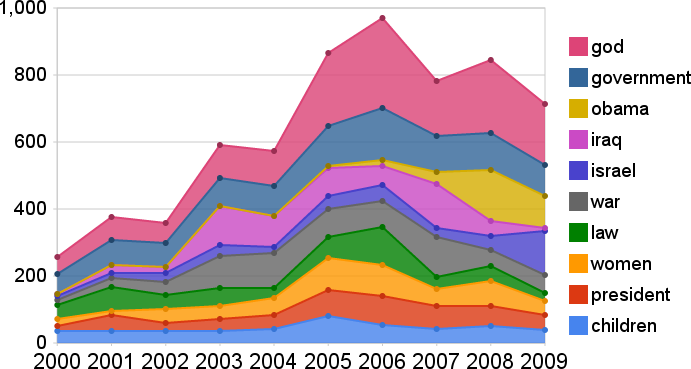
\includegraphics[width=8cm]{images/year_nouns.png}
	\caption{Frequency of different nouns on January 10th of various years}
	\label{year_nouns}
	\end{center}
\end{figure}


\todo{Lots of pretty graphs showing what our data is like.}

\subsection{Data Quality}

\x{Look at a random sample of the data and say how clean it is.}
\x{Evaluate the quality of the claims that we extracted.}
\x{Evaluate the quality of the clusters that we created.}
\x{Evaluate the quality of the different individual templates - which ones have the highest quality claims.}
\x{say something about {\em duplicate} claims?}


\subsection{Trends over time}

\x{Named entity recognition}

\x{Look at what noun phrases were most disputed at particular years.}
\x{Look at what noun phrases were most disputed on particular days.}

\x{We remove exact-match strings from the same domain - to avoid republishing of same article.}

\section{Conclusions}

Our research has shown that the web can be used as a corpus to determine what claims people identify as being disputed. Although it is likely that any specific claim found on the web is not authoritative, the web as a whole aggregates the array of views to be found online.

Furthermore, because individuals express opinions freely online, a snapshot of the disputed claims online can provide valuable insights into the cultural zeitgeist of the time.

Challenges of creating a comprehensive corpus of disputed claims are many, from data quality to deeper natural language processing challenges such as recognizing textual entailment. We address these in part by taking a high-level statistical view of the data.

The possible applications of a corpus of disputed claims are many and varied. These include real-time dispute recognition, autonomous research agents that operate in the background, and sociocultural research.

Using the claim prefix search technique and text processing, we are able to identify 

Our data set currently includes approximately 1.2 million records. We intend to expand this by several orders of magnitude, an improvement that will address issues of data sparsity and enable more robust data processing. 

%\section{Acknowledgments}

\todo{Do we want to have acknowledgements}
% We would like to Thank Barbara Rosario for help with textual entailment, and 
% Acknowledgements omitted for blind submission. Dispute Finder uses icons from the free FamFamFam Silk\footnote{http://famfamfam.com} collection.

% mendelybib is the bibliograph from our shared mendely space and is auto-generated
% localbib is used for manually adding anything we don't want to add to mendeley, particularly for
% people who are not mendeley users
\bibliography{mendeleybib,localbib}

\end{document}


